\documentclass[14pt]{beamer}
\usepackage{./Estilos/BeamerUVM}
\usepackage{./Estilos/ColoresLatex}
\usetheme{Madrid}
\usecolortheme{default}
%\useoutertheme{default}
\setbeamercovered{invisible}
% or whatever (possibly just delete it)
\setbeamertemplate{section in toc}[sections numbered]
\setbeamertemplate{subsection in toc}[subsections numbered]
\setbeamertemplate{subsection in toc}{\leavevmode\leftskip=3.2em\rlap{\hskip-2em\inserttocsectionnumber.\inserttocsubsectionnumber}\inserttocsubsection\par}
% \setbeamercolor{section in toc}{fg=blue}
% \setbeamercolor{subsection in toc}{fg=blue}
% \setbeamercolor{frametitle}{fg=blue}
\setbeamertemplate{caption}[numbered]

\setbeamertemplate{footline}
\beamertemplatenavigationsymbolsempty
\setbeamertemplate{headline}{}


\makeatletter
% \setbeamercolor{section in foot}{bg=gray!30, fg=black!90!orange}
% \setbeamercolor{subsection in foot}{bg=blue!30}
% \setbeamercolor{date in foot}{bg=black}
\setbeamertemplate{footline}
{
  \leavevmode%
  \hbox{%
  \begin{beamercolorbox}[wd=.333333\paperwidth,ht=2.25ex,dp=1ex,center]{section in foot}%
    \usebeamerfont{section in foot} {\insertsection}
  \end{beamercolorbox}%
  \begin{beamercolorbox}[wd=.333333\paperwidth,ht=2.25ex,dp=1ex,center]{subsection in foot}%
    \usebeamerfont{subsection in foot}  \insertsubsection
  \end{beamercolorbox}%
  \begin{beamercolorbox}[wd=.333333\paperwidth,ht=2.25ex,dp=1ex,right]{date in head/foot}%
    \usebeamerfont{date in head/foot} \insertshortdate{} \hspace*{2em}
    \insertframenumber{} / \inserttotalframenumber \hspace*{2ex} 
  \end{beamercolorbox}}%
  \vskip0pt%
}
\makeatother

\makeatletter
\patchcmd{\beamer@sectionintoc}{\vskip1.5em}{\vskip0.8em}{}{}
\makeatother

% \usefonttheme{serif}
\usepackage[clock]{ifsym}
\usetikzlibrary{plotmarks}

\sisetup{per-mode=symbol}
\resetcounteronoverlays{saveenumi}

\title{\Large{Cinemática} \\ \normalsize{Física 1}}
\date{3 de julio de 2023}

\begin{document}
\maketitle

\section*{Contenido}
\frame{\frametitle{Contenido} \tableofcontents[currentsection, hideallsubsections]}


\section{Trabajo de desarrollo}
\frame{\tableofcontents[currentsection, hideothersubsections]}
\subsection{Indicaciones}

\begin{frame}
\frametitle{Trabajo de desarrollo}
Deberás de realizar un trabajo con los siguientes puntos:
\pause
\setbeamercolor{item projected}{bg=bananayellow,fg=ao}
\setbeamertemplate{enumerate items}{%
\usebeamercolor[bg]{item projected}%
\raisebox{1.5pt}{\colorbox{bg}{\color{fg}\footnotesize\insertenumlabel}}%
}
\begin{enumerate}[<+->]
\item Un revisión biográfica de Isaac Newton y de Johannes Kepler.
\seti
\end{enumerate}
\end{frame}
\begin{frame}
\frametitle{Trabajo de desarrollo}
\setbeamercolor{item projected}{bg=bananayellow,fg=ao}
\setbeamertemplate{enumerate items}{%
\usebeamercolor[bg]{item projected}%
\raisebox{1.5pt}{\colorbox{bg}{\color{fg}\footnotesize\insertenumlabel}}%
}
\begin{enumerate}[<+->]
\conti
\item Para Isaac Newton deberás de presentar de manera general, las aportaciones que hizo para la mecánica, en particular, las llamadas Leyes de Newton, respondiendo ¿de qué manera logró establecer o construir esas leyes?
\seti
\end{enumerate}
\end{frame}
\begin{frame}
\frametitle{Trabajo de desarrollo}
\setbeamercolor{item projected}{bg=bananayellow,fg=ao}
\setbeamertemplate{enumerate items}{%
\usebeamercolor[bg]{item projected}%
\raisebox{1.5pt}{\colorbox{bg}{\color{fg}\footnotesize\insertenumlabel}}%
}
\begin{enumerate}[<+->]
\conti
\item Para Johannes Kepler, presentarás su trabajo conocido como las Leyes de Kepler, ¿en qué consisten? ¿qué fenómenos explican?
\seti
\end{enumerate}
\end{frame}
\begin{frame}
\frametitle{Trabajo de desarrollo}
\setbeamercolor{item projected}{bg=bananayellow,fg=ao}
\setbeamertemplate{enumerate items}{%
\usebeamercolor[bg]{item projected}%
\raisebox{1.5pt}{\colorbox{bg}{\color{fg}\footnotesize\insertenumlabel}}%
}
\begin{enumerate}[<+->]
\conti
\item Para entender las Leyes de Kepler, será necesario estudiar también el lugar geométrico llamado elipse. Pero no desde el punto de vista matemático, es decir, no hay que señalar la ecuación que la define, sino las propiedades o características que presenta una elipse.
\seti
\end{enumerate}
\end{frame}
\begin{frame}
\frametitle{Trabajo de desarrollo}
\setbeamercolor{item projected}{bg=bananayellow,fg=ao}
\setbeamertemplate{enumerate items}{%
\usebeamercolor[bg]{item projected}%
\raisebox{1.5pt}{\colorbox{bg}{\color{fg}\footnotesize\insertenumlabel}}%
}
\begin{enumerate}[<+->]
\conti
\item Deberás de presentar un método a partir del cual se puede construir una elipse en el cuaderno. Hay varias propuestas, pero la que elijas, deberás de presentar el desarrollo completo, de tal manera que muestres la manera en la que se obtiene.
\seti
\end{enumerate}
\end{frame}
\begin{frame}
\frametitle{Trabajo de desarrollo}
\setbeamercolor{item projected}{bg=bananayellow,fg=ao}
\setbeamertemplate{enumerate items}{%
\usebeamercolor[bg]{item projected}%
\raisebox{1.5pt}{\colorbox{bg}{\color{fg}\footnotesize\insertenumlabel}}%
}
\begin{enumerate}[<+->]
\conti
\item Esta actividad de desarrollo aportará hasta $10$ puntos de evaluación continua.
\item La evaluación se hará con una rúbrica, pero el nivel de calidad y exigencia del trabajo será mayor.
\seti
\end{enumerate}
\end{frame}
\begin{frame}
\frametitle{Trabajo de desarrollo}
\setbeamercolor{item projected}{bg=bananayellow,fg=ao}
\setbeamertemplate{enumerate items}{%
\usebeamercolor[bg]{item projected}%
\raisebox{1.5pt}{\colorbox{bg}{\color{fg}\footnotesize\insertenumlabel}}%
}
\begin{enumerate}[<+->]
\conti
\item La entrega del trabajo será por Teams, el plazo para el envío es el día 5 de julio a las 8 pm.
\item No se recibirán trabajos extemporáneos, a menos que se presente la evidencia de problemas técnicos durante el envío y que se haya notificado oportunamente a la Coordinación Académica y al Profesor.
\end{enumerate}
\end{frame}

\section{Ejercicios de recuperación}
\frame{\tableofcontents[currentsection, hideothersubsections]}
\subsection{Trabajo a resolver}

\begin{frame}
\frametitle{Objetivo del Trabajo}
Con la finalidad de apoyar en la recuperación del promedio para los siguientes exámenes parciales, \pause se dejarán una serie de \textocolor{red}{ejercicios adicionales} para Evaluación Continua.
\end{frame}
\begin{frame}
\frametitle{Ejercicios opcionales}
Estos ejercicios serán de carácter \textocolor{cobalt}{opcional}, \pause es decir, la alumna o alumno que desee resolverlos y enviarlos, les sumará $5$ puntos adicionales a la Evaluación Continua.
\end{frame}
\begin{frame}
\frametitle{Puntaje adicional}
Si por ejemplo, para el segundo parcial se tienen 20 puntos de Evaluación Continua, \pause al sumar $5$ puntos adicionales, el puntaje se calculará sobre los $20$ ejercicios, \pause por decir: \pause $25/20$ de puntaje.
\end{frame}
\begin{frame}
\frametitle{Puntaje y calificación de teoría}
Ese puntaje de Evaluación Continua corresponde al $50\%$ de la calificación de teoría, \pause lo que ayudaría a subir el promedio del segundo parcial.
\end{frame}
\begin{frame}
\frametitle{Ventaja para la calificación}
Quien desee resolver y enviar los ejercicios, podrá mejorar su promedio para el siguiente parcial.
\\
\bigskip
Lo que es completamente atractivo para mejorar la calificación del curso.
\end{frame}
\begin{frame}
\frametitle{Fecha de entrega}
Los ejercicios adicionales se dejarán cada semana, \pause debiendo de entregarse el día domingo a las 8 pm.
\end{frame}
\begin{frame}
\frametitle{Aviso importante}
Los ejercicios adicionales NO sustituyen a los ejercicios de Evaluación Continua que se dejarán.
\\
\bigskip
\pause
Si alguien decide no enviar los ejercicios adicionales, no tendrá penalización alguna.
\end{frame}

\section{Cinemática}
\frame{\tableofcontents[currentsection, hideothersubsections]}
\subsection{Conceptos}

\begin{frame}
\frametitle{¿Qué es la mecánica?}
La \textocolor{ao}{mecánica} es la rama de la Física que se encarga del estudio de los cuerpos en movimiento; \pause se divide en \pause \textocolor{burgundy}{cinemática} \pause y \textocolor{darkgreen}{dinámica}.
\end{frame}
\begin{frame}
\frametitle{Cinemática}
La cinemática es la parte de la mecánica que estudia los diferentes tipos de movimiento de los objetos sin atender las causas que lo produjeron.
\end{frame}
\begin{frame}
\frametitle{Movimiento}
Es el cambio de lugar que experimenta un cuerpo dentro de un espacio determinado.
\end{frame}
\begin{frame}
\frametitle{Sistema de referencia}
Sistema de elementos que sirve para fijar la posición de un cuerpo en movimiento.
\end{frame}
\begin{frame}
\frametitle{Posición}
Es el lugar físico en el que se encuentra un cuerpo dentro de un espacio determinado.
\end{frame}
\begin{frame}
\frametitle{Distancia}
La distancia recorrida por un móvil es una \textocolor{magenta}{magnitud escalar}, \pause ya que sólo interesa saber cuál fue la magnitud de la longitud recorrida por el móvil durante la trayectoria seguida, sin importar en qué dirección lo hizo.
\end{frame}
\begin{frame}
\frametitle{Trayectoria}
Es la línea que une las diferentes posiciones que a medida que pasa el tiempo va ocupando un punto en el espacio o, de otra forma, es el camino que sigue el objeto dentro de un movimiento.
\end{frame}
\begin{frame}
\frametitle{Trayectoria}
\begin{figure}
    \centering
    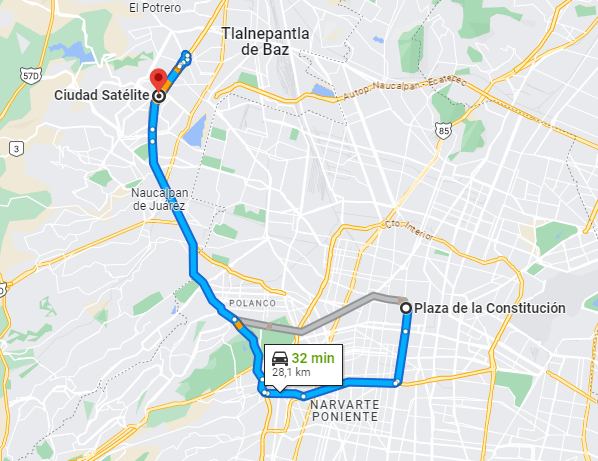
\includegraphics[scale=0.45]{Imagenes/Trayectoria_01.png}
\end{figure}
\end{frame}
\begin{frame}
\frametitle{Tipos de Trayectoria}
Cuando la trayectoria es una línea recta se dice que el movimiento es rectilíneo.
\\
\bigskip
\pause
Cuando la trayectoria es un círculo decimos que el movimiento es circular.
\end{frame}
\begin{frame}
\frametitle{Desplazamiento}
El desplazamiento de un móvil es una \textocolor{cerise}{magnitud vectorial}, ya que corresponde a una distancia medida en una dirección particular entre dos puntos: el de partida y el de llegada.
\end{frame}
\begin{frame}
\frametitle{Desplazamiento}
\begin{figure}
    \centering
    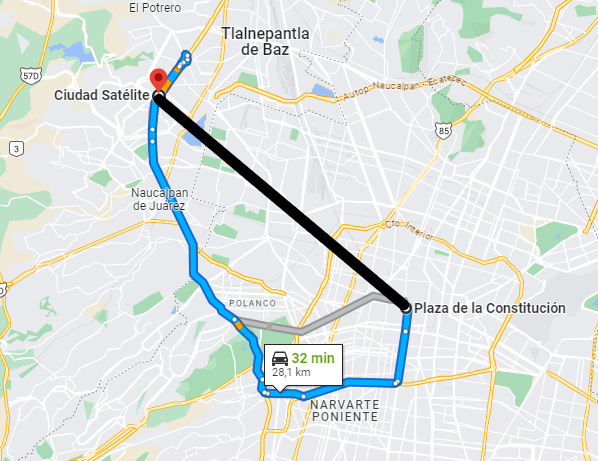
\includegraphics[scale=0.45]{Imagenes/Trayectoria_02.png}
\end{figure}
\end{frame}

\section{Movimiento Rectilíneo Uniforme}
\frame{\tableofcontents[currentsection, hideothersubsections]}
\subsection{Conceptos relevantes}

\begin{frame}
\frametitle{Rapidez}
La \textocolor{auburn}{rapidez} es la distancia recorrida por un objeto en cierto tiempo.
\\
\bigskip
\pause
Es una \textocolor{awesome}{cantidad escalar}, porque se define con una magnitud y una unidad de medida.
\end{frame}
\begin{frame}
\frametitle{Expresión para la rapidez}
La rapidez se obtiene mediante la siguiente expresión:
\pause
\begin{align*}
\text{rapidez} = \dfrac{\text{distancia}}{\text{tiempo}}
\end{align*}
Las unidades son metros por segundo (\unit[per-mode=symbol]{\meter\per\second})
\end{frame}
\begin{frame}
\frametitle{Velocidad}
Es la razón de cambio del desplazamiento de un objeto con respecto al tiempo.
\\
\bigskip
\pause
La velocidad es una \textocolor{byzantine}{magnitud vectorial}.
\end{frame}
\begin{frame}
\frametitle{Expresión para la velocidad}
La velocidad se obtiene mediante la siguiente expresión:
\pause
\begin{eqnarray*}
\begin{aligned}
\text{velocidad} = \dfrac{\text{desplazamiento}}{\text{tiempo}} \pause \hspace*{1.5cm} v = \dfrac{d}{t}
\end{aligned}
\end{eqnarray*}
\pause
Las unidades de la velocidad son metros por segundo (\unit[per-mode=symbol]{\meter\per\second})
\end{frame}
\begin{frame}
\frametitle{Velocidad final}
Es el último instante o momento de la distancia recorrida en el tiempo.
\end{frame}
\begin{frame}
\frametitle{Velocidad media}
Promedio de la suma de todas las distancias y tiempos recorridos.
\end{frame}
\begin{frame}
\frametitle{El triángulo de la velocidad}
En física es común apoyarse con ciertas reglas de tipo visual, que nos ayudarán a simplificar el manejo de una expresión.
\\
\bigskip
\pause
Tal es el caso del \textbf{Triángulo de la velocidad}.
\end{frame}
\begin{frame}
\frametitle{El triángulo de la velocidad}
\begin{figure}
\centering
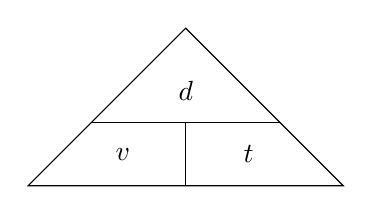
\begin{tikzpicture}
    \draw (0, 0) -- (4, 0) -- (2, 2) -- cycle;
    \draw (2, 0) -- (2, 0.8);
    \draw (0.8, 0.8) -- (3.2, 0.8);

    \node at (2, 1.2) {$d$};
    \node at (1.2, 0.4) {$v$};
    \node at (2.8, 0.4) {$t$};
\end{tikzpicture}
\end{figure}
La idea con esta imagen es recuperar de la expresión, la operación que se necesite si nos piden alguna de las tres variables.
\end{frame}
\begin{frame}
\frametitle{Ejercicio de velocidad}
Un corredor avanza \SI{2}{\kilo\meter} en un tiempo de \SI{15}{\minute}.
\\
\bigskip
\pause
Calcula su velocidad en \unit[per-mode=symbol]{\kilo\meter\per\hour} y en \unit[per-mode=symbol]{\meter\per\second}.
\pause
Revisa que nos piden hacer una conversión de unidades.
\end{frame}
\begin{frame}
\frametitle{Primer paso para la solución al ejercicio}
Se recomienda siempre tener los \textocolor{red}{datos} que nos indica el enunciado.
\pause
\begin{eqnarray*}
\begin{aligned}
\text{desplazamiento} &= \SI{2}{\kilo\meter} \\[0.5em] \pause
\text{tiempo} &= \SI{15}{\minute}
\end{aligned}
\end{eqnarray*}
\end{frame}
\begin{frame}
\frametitle{Segundo paso para la solución al ejercicio}
Nos conviene anotar la \textocolor{cadmiumgreen}{expresión} a utilizar, ya sea de uso directo o tengamos que despejar alguna variable. \pause Nos apoyamos con el triángulo de la velocidad:
\pause
\begin{figure}
\centering
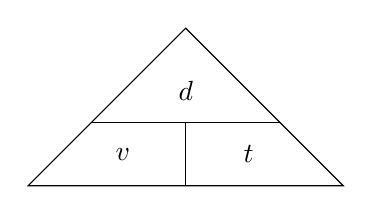
\begin{tikzpicture}
    \draw (0, 0) -- (4, 0) -- (2, 2) -- cycle;
    \draw (2, 0) -- (2, 0.8);
    \draw (0.8, 0.8) -- (3.2, 0.8);

    \node at (2, 1.2) {$d$};
    \node at (1.2, 0.4) {$v$};
    \node at (2.8, 0.4) {$t$};
\end{tikzpicture}
\end{figure}        
\end{frame}
\begin{frame}
\frametitle{Tercer paso para la solución al ejercicio}
Hacemos la sustitución con los valores que nos indica el enunciado:
\pause
\begin{eqnarray*}
\begin{aligned}
v = \dfrac{\SI{2}{\kilo\meter}}{\SI{15}{\minute}} = \pause \SI[per-mode=fraction]{0.1333}{\kilo\meter\per\minute}
\end{aligned}
\end{eqnarray*}
\pause
Nos falta hacer la conversión de unidades.
\end{frame}
\begin{frame}
\frametitle{Haciendo la conversión de unidades}
\begin{eqnarray*}
\begin{aligned}
v &= \SI[per-mode=fraction]{0.1333}{\kilo\meter\per\minute} \left( \dfrac{\SI{60}{\minute}}{\SI{1}{\hour}} \right) = \pause \SI[per-mode=fraction]{8}{\kilo\meter\per\hour} \\[0.5em] \pause
v &= \SI[per-mode=fraction]{0.1333}{\kilo\meter\per\minute} \left( \dfrac{\SI{d3}{\meter}}{\SI{1}{\kilo\meter}} \right) \left( \dfrac{\SI{1}{\hour}}{\SI{3.6d2}{\second}} \right)  = \pause \SI[per-mode=fraction]{2.22}{\meter\per\second}
\end{aligned}
\end{eqnarray*}
\end{frame}
\begin{frame}
\frametitle{Otro ejercicio}
Un ciclista puede alcanzar en una bajada una velocidad de hasta \SI{35}{\kilo\meter\per\hour}.
\\
\bigskip
\pause
¿Qué distancia recorre en una pendiente después de \SI{2}{\minute}?
\end{frame}
\begin{frame}
\frametitle{Datos del enunciado}
\begin{eqnarray*}
\begin{aligned}
v &= \SI{35}{\kilo\meter\per\hour} \\[0.5em] \pause
t &= \SI{2}{\minute} \\[0.5em] \pause
d &= \, ?
\end{aligned}
\end{eqnarray*}
\end{frame}
\begin{frame}
\frametitle{Expresión a utilizar}
\begin{figure}
\centering
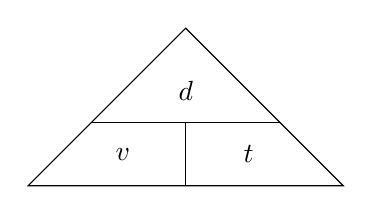
\begin{tikzpicture}
    \draw (0, 0) -- (4, 0) -- (2, 2) -- cycle;
    \draw (2, 0) -- (2, 0.8);
    \draw (0.8, 0.8) -- (3.2, 0.8);

    \node at (2, 1.2) {$d$};
    \node at (1.2, 0.4) {$v$};
    \node at (2.8, 0.4) {$t$};
\end{tikzpicture}
\end{figure}        
\begin{align*}
d = v \, t
\end{align*}
\end{frame}
\begin{frame}
\frametitle{Conversión de unidades}
Antes de hacer la sustitución, debemos de hacer una conversión de unidades para mantener la congruencia con el resultado:
\pause
\begin{eqnarray*}
\begin{aligned}
\SI[per-mode=fraction]{35}{\kilo\meter\per\hour} \left( \dfrac{\SI{d3}{\meter}}{\SI{1}{\kilo\meter}} \right) \left( \dfrac{\SI{1}{\hour}}{\SI{60}{\minute}} \right) = \pause \SI[per-mode=fraction]{583.3}{\meter\per\minute}
\end{aligned}
\end{eqnarray*}
\end{frame}
\begin{frame}
\frametitle{Conversión de unidades}
Ahora sustituimos los valores que ya hemos convertido:
\pause
\begin{eqnarray*}
\begin{aligned}
d &= v \, t \pause = \left( \SI[per-mode=fraction]{583.3}{\meter\per\minute} \right) \left( \SI{2}{\minute} \right) = \\[0.5em] \pause
d &= \SI{1166.6}{\meter}
\end{aligned}
\end{eqnarray*}
\end{frame}
\begin{frame}
\frametitle{Otro ejercicio}
Un auto viaja en una carretera a una velocidad constante de \SI{120}{\kilo\meter\per\hour}
\\
\bigskip
\pause
¿Cuánto tiempo le tomará llegar al poblado más cercano, que está a \SI{180}{\kilo\meter} a esa misma velocidad?
\end{frame}
\begin{frame}
\frametitle{Resolviendo el ejercicio}
\textocolor{red}{Datos:}
\pause
\begin{align*}
v &= \SI{120}{\kilo\meter\per\hour} \\[0.5em]
d &= \SI{180}{\kilo\meter} \\[0.5em]
t &= \, ?
\end{align*}
\end{frame}
\begin{frame}
\frametitle{Resolviendo el ejercicio}
\textocolor{red}{Expresión:}
\pause
\begin{eqnarray*}
\begin{aligned}
v &= \dfrac{d}{t} \\[0.5em] \pause
t &= \dfrac{d}{v}
\end{aligned}
\end{eqnarray*}
\end{frame}
\begin{frame}
\frametitle{Resolviendo el ejercicio}
\textocolor{red}{Sustitución:} Una vez conocida la expresión que debemos de ocupar, procedemos a sustituir los valores que nos indica el enunciado.
\pause
\begin{eqnarray*}
\begin{aligned}
t &= \dfrac{v}{d} \\[0.5em] \pause
t &= \dfrac{\SI{180}{\kilo\meter}}{\SI{120}{\kilo\meter\per\hour}} = \\[0.5em] \pause
t &= \SI{1.5}{\hour}
\end{aligned}
\end{eqnarray*}
\end{frame}
\begin{frame}
\frametitle{Ejercicios de Evaluación Continua}
Con la finalidad de practicar la expresión para la velocidad, desplazamiento y tiempo, se dejarán $6$ ejercicios que contarán como Evaluación Continua, el puntaje a obtener son $6$ puntos.
\end{frame}
\begin{frame}
\frametitle{Ejercicios de Evaluación Continua}
Los ejercicios estarán en un documento en la asignación en Teams, el plazo de entrega es para el domingo 9 de julio a las 8 pm.
\end{frame}

\subsection{Intepretando una gráfica}

\begin{frame}
\frametitle{La utilidad de una gráfica}
El movimiento de un cuerpo se puede representar de manera oportuna mediante una gráfica, \pause por lo que será conveniente revisar la manera en la que podemos \enquote{leer} la información contenida en esa gráfica.
\end{frame}
\begin{frame}
\frametitle{El eje horizontal}
Comenzamos reconociendo que en el \textocolor{cadetblue}{eje de las abscisas} tendremos siempre la \textocolor{magenta}{variable temporal}, es decir, el tiempo $t$.
\\
\bigskip
\pause
El tiempo será la \textocolor{alizarin}{variable independiente}.
\end{frame}
\begin{frame}
\frametitle{El eje vertical}
En el \textocolor{ballblue}{eje de las ordenadas}, tendremos la variable de \textocolor{auburn}{desplazamiento}.
\\
\bigskip
\pause
El desplazamiento será la \textocolor{burntumber}{variabe dependiente}.
\end{frame}
\begin{frame}
\frametitle{La base de la gráfica}
\begin{figure}
    \centering
    \begin{tikzpicture}
        \draw (0, 0) -- (7.5, 0) node [above, pos=1] {\small{$t \, [\unit{\second}]$}};
        \draw (0, 0) -- (0, 5.3) node [left, pos=1.1] {\small{$d \, [\unit{\meter}]$}};

        \pause

        \foreach [evaluate={\j=int(\x*10)}] \x in {1, 2, 3, 4, 5, 6, 7}
        {    
            \draw (\x, 0.2) -- (\x, -0.2);
            \node at (\x, -0.4) {\small{$\x$}};
        }
        \foreach [evaluate={\j=int(\x*10)}] \x in {1, 2, 3, 4, 5}
        {
            \draw (-0.2, \x) -- (0.2, \x);
            \node at (-0.6, \x) {\small{$\j$}};
        }
        \pause
        \draw [thick, color=ao] (0, 0) -- (1, 1); \pause
        \draw [thick, color=ao] (1, 1) -- (3, 2); \pause
        \draw [thick, color=ao] (3, 2) -- (4, 4); \pause
        \draw [thick, color=ao] (4, 4) -- (5, 5); \pause
        \draw [thick, color=ao] (5, 5) -- (7, 5); \pause
    \end{tikzpicture}
\end{figure}
\end{frame}


\section{Movimiento uniformemente acelerado}
\frame{\tableofcontents[currentsection, hideothersubsections]}
\subsection{La aceleración}

\begin{frame}
\frametitle{Construyendo la aceleración}
Supongamos que un cuerpo se mueve a lo largo de una línea recta y cada segundo se registra que su velocidad aumenta (o disminuye) en \SI{10}{\meter\per\second}.
\end{frame}
\begin{frame}
\frametitle{Construyendo la aceleración}
De manera que al segundo $1$ su velocidad es de \SI{10}{\meter\per\second}, \pause al segundo $2$ es de \SI{20}{\meter\per\second}, \pause al segundo $3$ es \SI{30}{\meter\per\second}, \pause al segundo $4$ es \SI{40}{\meter\per\second}, \pause y por último al segundo $5$, su velocidad es \SI{50}{\meter\per\second}
\end{frame}
\begin{frame}
\frametitle{Preparando una tabla}
\begin{table}
\renewcommand{\arraystretch}{1}
\centering
\begin{tabular}{c | c}
Tiempo [\unit{\second}] & Velocidad [\unit{\meter\per\second}] \\ \hline
$1$ & $10$ \\ \hline
$2$ & $20$ \\ \hline
$3$ & $30$ \\ \hline
$4$ & $40$ \\ \hline
$5$ & $50$ \\ \hline
\end{tabular}
\end{table}
\end{frame}
\begin{frame}
\frametitle{Graficando el cambio de velocidad}
\begin{figure}
    \centering
    \begin{tikzpicture}
        \draw (0, 0) -- (6, 0) node [above, pos=1] {\small{$t \, [\unit{\second}]$}};
        \draw (0, 0) -- (0, 5.3) node [left, pos=1.1] {\small{$v \, [\unit{\meter\per\second}]$}};

        \foreach [evaluate={\j=int(\x*10)}] \x in {1, 2, 3, 4, 5}
            {    
            \draw (\x, 0.2) -- (\x, -0.2);
            \node at (\x, -0.4) {\small{$\x$}};

            \draw (-0.2, \x) -- (0.2, \x);
            \node at (-0.6, \x) {\small{$\j$}};
            }

            \foreach \x in {1, 2, 3, 4, 5}
                {
                    \draw [color=blue, fill] (\x, \x) circle (0.4mm);
                    \draw [dashed] (\x, 0) -- (\x, \x);
                    \draw [dashed] (0, \x) -- (\x, \x); \pause
                }
    \end{tikzpicture}
\end{figure}
\end{frame}
\begin{frame}
\frametitle{titulo}
\frametitle{Graficando el cambio de velocidad}
\begin{figure}
    \centering
    \begin{tikzpicture}
        \draw (0, 0) -- (6, 0) node [above, pos=1] {\small{$t \, [\unit{\second}]$}};
        \draw (0, 0) -- (0, 5.3) node [left, pos=1.1] {\small{$v \, [\unit{\meter\per\second}]$}};

        \foreach [evaluate={\j=int(\x*10)}] \x in {1, 2, 3, 4, 5}
            {    
            \draw (\x, 0.2) -- (\x, -0.2);
            \node at (\x, -0.4) {\small{$\x$}};

            \draw (-0.2, \x) -- (0.2, \x);
            \node at (-0.6, \x) {\small{$\j$}};
            }

        \foreach \x in {1, 2, 3, 4, 5}
            \draw [color=blue, fill] (\x, \x) circle (0.4mm);

        \draw [thick, red] (1, 1) -- (5, 5);

    \end{tikzpicture}
\end{figure}
\end{frame}
\begin{frame}
\frametitle{Construyendo la aceleración}
Con estos valores reconocemos que la velocidad está variando en \SI{10}{\meter\per\second} cada \SI{1}{\second}, \pause esto es, el cuerpo tiene una aceleración de \SI{10}{\meter\per\square\second}
\end{frame}
\begin{frame}
\frametitle{La aceleración}
Se define la \textocolor{red}{aceleración} \pause como la razón de cambio de la velocidad con respecto al tiempo.
\\
\bigskip
\pause
Es una \textocolor{cerise}{cantidad vectorial}, porque consta de un magnitud o valor, dirección y sentido.
\end{frame}
\begin{frame}
\frametitle{Expresión para la aceleración}
\begin{eqnarray*}
\begin{aligned}
a &= \dfrac{\text{cambio de velocidad}}{\text{intervalo de tiempo}} = \pause \dfrac{\Delta \, v}{\Delta \, t} = \\[1em] \pause
a &= \dfrac{\text{Velocidad final - Velocidad inicial}}{\text{tiempo}} = \\[1em] \pause
a &= \dfrac{v_{f} - v_{i}}{t}
\end{aligned}
\end{eqnarray*}
\end{frame}
\begin{frame}
\frametitle{Consideraciones}
La \textocolor{cobalt}{velocidad inicial} ($v_{i}$) del objeto se define como la velocidad del móvil al inicio del intervalo de tiempo, \pause y que si el objeto se encuentra \textocolor{byzantine}{en reposo}, esta velocidad tiene un valor de cero.
\end{frame}
\begin{frame}
\frametitle{Consideraciones}
La \textocolor{bole}{velocidad final} ($v_{f}$) se define como la velocidad al terminar el intervalo de tiempo.
\end{frame}
\begin{frame}
\frametitle{Signo de la aceleración}
Se considera que un móvil tiene una \textocolor{darkgreen}{aceleración positiva} cuando aumenta su velocidad.
\\
\bigskip
\pause
Si disminuye su velocidad tiene \textocolor{blue-violet}{aceleración negativa} (desaceleración o frenado).
\end{frame}
\begin{frame}
\frametitle{Aceleración nula}
De igual modo se considera que un cuerpo no tiene aceleración ($a = 0$) si \textbf{está inmóvil} \pause o si se mueve con \textbf{velocidad constante} ($a = 0$).
\end{frame}

\subsection{Aceleración constante}

\begin{frame}
\frametitle{Tipo de problemas}
Cuando se resuelven problemas donde esté involucrada una \textocolor{red}{aceleración constante}, \pause es importante elegir la fórmula correcta y sustituir los datos conocidos.
\end{frame}
\begin{frame}
\frametitle{Tipo de problemas}
Los problemas se refieren frecuentemente al movimiento de un móvil que \textocolor{ao}{parte del reposo} o que \textocolor{cadmiumgreen}{se detiene} después de cierta velocidad.
\end{frame}
\begin{frame}
\frametitle{Expresiones más utilizadas}
Las siguientes son las fórmulas más utilizadas en el movimiento uniformemente acelerado:
\end{frame}
\begin{frame}
\frametitle{La aceleración como función del tiempo}
Conociendo la velocidad final $v_{f}$, la velocidad inicial $v_{i}$ y el tiempo $t$, calculamos la aceleración del objeto:
\pause
\begin{align*}
a = \dfrac{v_{f} - v_{i}}{t} \hspace*{1.5cm} \left[ \dfrac{\unit{\meter}}{\unit{\square\second}} \right]
\end{align*}
\end{frame}
\begin{frame}
\frametitle{La aceleración como función del desplazamiento}
Conociendo la velocidad final $v_{f}$, la velocidad inicial $v_{i}$ y el desplazamiento $d$, calculamos la aceleración del objeto:
\pause
\begin{align*}
a = \dfrac{v_{f}^{2} - v_{i}^{2}}{2 \, d} \hspace*{1.5cm} \left[ \dfrac{\unit{\meter}}{\unit{\square\second}} \right]
\end{align*}
\end{frame}
\begin{frame}
\frametitle{El desplazamiento como función del tiempo}
Conociendo la velocidad final $v_{f}$, la velocidad inicial $v_{i}$ y el tiempo $t$, calculamos el desplazamiento que recorre el objeto:
\pause
\begin{align*}
d = \left( \dfrac{v_{f} + v_{i}}{2} \right) \, t \hspace*{1.5cm} \left[ \unit{\meter} \right]
\end{align*}
\end{frame}
\begin{frame}
\frametitle{El desplazamiento como función de la aceleración}
Conociendo la la velocidad inicial $v_{i}$, la aceleración $a$ y el tiempo $t$, calculamos el desplazamiento que recorre el objeto:
\pause
\begin{align*}
d = v_{i} \, t + \dfrac{1}{2} \, a \, t^{2} \hspace*{1.5cm} \left[ \unit{\meter} \right]
\end{align*}
\end{frame}
\begin{frame}
\frametitle{Ejercicio}
Un autobús viaja en una carretera a una velocidad de \SI{70}{\kilo\meter\per\hour} y acelera durante \SI{30}{\second} hasta llegar a su límite de velocidad, que son \SI{95}{\kilo\meter\per\hour}.
\\
\bigskip
\pause
¿Cuál fue su aceleración?
\end{frame}
\begin{frame}
\frametitle{Solución al ejercicio}
\textocolor{red}{Datos:}
\begin{align*}
v_{i} &= \SI{70}{\kilo\meter\per\hour} \\[0.5em]
v_{f} &= \SI{95}{\kilo\meter\per\hour} \\[0.5em]
t &= \SI{30}{\second} \\[0.5em]
a &= \, ?
\end{align*}
\end{frame}
\begin{frame}
\frametitle{Resolviendo el ejercicio}
\textocolor{red}{Expresión}:
\pause
\begin{align*}
a = \dfrac{v_{f} - v_{i}}{t}
\end{align*}
\pause
\textocolor{red}{Conversión de unidades:}
\begin{eqnarray*}
\begin{aligned}
v_{i} &= \left( \SI[per-mode=fraction]{70}{\kilo\meter\per\hour} \right) \left( \dfrac{\SI{1000}{\meter}}{\SI{1}{\kilo\meter}} \right) \left( \dfrac{\SI{1}{\hour}}{\SI{3600}{\second}} \right) = \pause \SI[per-mode=fraction]{19.44}{\meter\per\second}
\end{aligned}
\end{eqnarray*}
\end{frame}
\begin{frame}
\frametitle{Resolviendo el ejercicio}
\textocolor{red}{Conversión de unidades:}
\begin{eqnarray*}
\begin{aligned}
v_{f} &= \left( \SI[per-mode=fraction]{95}{\kilo\meter\per\hour} \right) \left( \dfrac{\SI{1000}{\meter}}{\SI{1}{\kilo\meter}} \right) \left( \dfrac{\SI{1}{\hour}}{\SI{3600}{\second}} \right) = \pause \SI[per-mode=fraction]{26.36}{\meter\per\second}
\end{aligned}
\end{eqnarray*}
\end{frame}
\begin{frame}
\frametitle{Resolviendo el ejercicio}
\textocolor{red}{Sustitución:}
\begin{eqnarray*}
\begin{aligned}
a = \dfrac{\SI[per-mode=fraction]{26.36}{\meter\per\second} - \SI[per-mode=fraction]{19.44}{\meter\per\second}}{\SI{30}{\second}} = \pause \SI[per-mode=fraction]{0.23}{\meter\per\square\second}
\end{aligned}
\end{eqnarray*}
\end{frame}
\begin{frame}
\frametitle{Ejercicio 2}
Una tren viaja a una velocidad de \SI{32}{\meter\per\second} y se detiene por completo después de haber recorrido \SI{140}{\meter}
\\
\bigskip
\pause
¿Cuál fue su aceleración y en cuánto tiempo se detuvo?
\end{frame}
\begin{frame}
\frametitle{Solución al ejercicio}
El enunciado nos pide dos cosas:
\setbeamercolor{item projected}{bg=black,fg=white}
\setbeamertemplate{enumerate items}{%
\usebeamercolor[bg]{item projected}%
\raisebox{1.5pt}{\colorbox{bg}{\color{fg}\footnotesize\insertenumlabel}}%
}
\begin{enumerate}[<+->]
\item La aceleración $a$.
\item El tiempo que tarda en detenerse.
\end{enumerate}
\pause Este tipo de ejercicios requiere de dos expresiones.
\end{frame}
\begin{frame}
\frametitle{Resolviendo el ejercicio}
\textocolor{red}{Datos:}
\begin{align*}
v_{i} &= \SI{32}{\meter\per\second} \\[0.4em] \pause
v_{f} &= 0 \\[0.4em]
d &= \SI{140}{\meter} \\[0.4em]
a &= \, ? \\[0.4em]
t &= \, ?
\end{align*}
\end{frame}
\begin{frame}
\frametitle{Resolviendo el ejercicio}
\textocolor{red}{Expresiones a utilizar}
\pause
\begin{eqnarray*}
\begin{aligned}
a &= \dfrac{v_{f}^{2} - v_{i}^{2}}{2 \, d} \\[0.5em] \pause
d &= \left( \dfrac{v_{f} + v_{i}}{2} \right) \, t \\[0.5em] \pause
t &= \pause \dfrac{2 \, d}{v_{f} + v_{i}}
\end{aligned}
\end{eqnarray*}
\end{frame}
\begin{frame}
\frametitle{Resolviendo el ejercicio}
\textocolor{red}{Sutitución:}
\pause
\begin{eqnarray*}
\begin{aligned}
a = \dfrac{ \left( \SI{0}{\meter\per\second} \right)^{2} - \left( \SI{32}{\meter\per\second} \right)^{2} }{2 ( \SI{140}{\meter})} = \pause - \SI{3.66}{\meter\per\square\second}
\end{aligned}
\end{eqnarray*}
El signo negativo nos indica que hay una desaceleración o frenado.
\end{frame}
\begin{frame}
\frametitle{Resolviendo el ejercicio}
\textocolor{red}{Sustitución:}
\pause
\begin{eqnarray*}
\begin{aligned}
t = \dfrac{2 (\SI{140}{\meter})}{\SI{32}{\meter\per\second} - \SI{0}{\meter\per\second}} = \pause \SI{8.75}{\second}
\end{aligned}
\end{eqnarray*}
\end{frame}

\section{Sobre el examen}
\frame[allowframebreaks]{\tableofcontents[currentsection, hideothersubsections]}
\subsection{Plan de recuperación}

\begin{frame}
\frametitle{Seguimento puntual}
Se ha iniciado un seguimiento puntual de las entregas de actividades de evaluación continua y de reportes de prácticas.
\end{frame}
\begin{frame}
\frametitle{Inasistencias}
Se informará de manera individual el número de inasistencias en la clase de Física 1 en conjunto con la clase de Laboratorio.
\\
\bigskip
\pause
A menos que se tenga una validación por parte de la Coordinación Académica, se modificará en el acta.
\end{frame}
\begin{frame}
\frametitle{Actividades pendientes}
A partir de hoy se recibirán actividades pendientes de enviar, \pause se calificarán \textocolor{red}{sobre 7 (siete)}, esto les dará un puntaje que es conveniente tener para sumar puntos.
\end{frame}
\begin{frame}
\frametitle{Plazo de entrega}
Se recibirán las actividades tanto de Evaluación Continua como reportes de Laboratorio, a más tardar el sábado 15 de julio de 2023 a las 8 pm.
\end{frame}
\begin{frame}
\frametitle{Plazo de entrega}
El envío se hará por mensaje directo en Teams al Profesor. Quienes tengan un seguimiento puntual, deberán enviar por el chat con la Coordinadora y Orientadora.
\end{frame}
\begin{frame}
\frametitle{De los reportes de prácticas pendientes}
Quien no haya asistido a una clase de Laboratorio, como tal, aparte de la inasistencia, no se le recibirá el trabajo que haya hecho el equipo el día de clase.
\end{frame}
\begin{frame}
\frametitle{Recuperación de Laboratorio}
Para obtener un puntaje en Laboratorio, se pide que quienes no tengan envío del reporte de las prácticas, \pause deberán de elaborar lo siguiente:
\end{frame}
\begin{frame}
\frametitle{Recuperación Práctica 3}
En el caso de la Práctica 3 Vectores, \pause deberán de resolver el ejercicio que se indica en el documento que se dejará en el grupo de Física 1.
\end{frame}
\begin{frame}
\frametitle{Recuperación Práctica 4}
En el caso de la Práctica 4 MRU, \pause deberán de resolver el mismo ejercicio de las tres corredoras, tal como se indicó en el material de la Práctica.
\end{frame}
\begin{frame}
\frametitle{Puntaje de recuperación}
Cada actividad de Laboratorio, se calificará \textocolor{ao}{sobre 7 (siete)}.
\end{frame}

\subsection{Retroalimentación}

\begin{frame}
\frametitle{Sesiones de Retroalimentación}
Se manejará como en la evaluación anterior, luego del examen se tendrá una sesión en donde se presentará la calificación del segundo examen parcial, así como de sus componentes.
\end{frame}
\begin{frame}
\frametitle{Inconformidades}
En caso de que manifiesten una inconformidad en su calificación, se les pide que presenten sus evidencias y argumentos para que en un plazo de 24 horas, quede resuelta su petición.
\end{frame}
\begin{frame}
\frametitle{Actividad opcional de Evaluación Continua}
Previo a la semana de exámenes, se te pide elabores \textocolor{darkblue}{por escrito} una guía con los temas, conceptos y expresiones que se presentaron del 26 de julio a la clase de hoy.
\end{frame}
\begin{frame}
\frametitle{Actividad opcional de Evaluación Continua}
Se abrirá una asignación para recibir el trabajo.
\\
\bigskip
\pause
El plazo vence el domingo 16 de julio a las 8 pm. \textocolor{burgundy}{Te otorgará un punto opcional}.
\end{frame}
\begin{frame}
\frametitle{Como dice la mercadotecnia}
\begin{figure}
    \centering
    
\includegraphics[scale=0.5]{Imagenes/Julio_Regalado.png}
\end{figure}
\end{frame}

\section{Caída libre}
\frame[allowframebreaks]{\frametitle{Temas a revisar}  \tableofcontents[currentsection, hideothersubsections]}
\subsection{Definición}

\begin{frame}
\frametitle{Planteando el escenario}
Es bien sabido que, en ausencia de resistencia del aire, \pause todos los objetos que se dejan caer cerca de la superficie de la Tierra caen hacia ella con la misma aceleración constante bajo la influencia de la gravedad de la Tierra.
\end{frame}
\begin{frame}
\frametitle{¿Caída libre?}
Cuando se usa la expresión objeto en \textocolor{ao}{caída libre} no necesariamente se hace referencia a
un objeto que se suelta desde el reposo.
\end{frame}
\begin{frame}
\frametitle{Influencia de la gravedad}
Un objeto en caída libre es cualquier objeto que se mueve libremente sólo bajo la \textocolor{red}{influencia de la gravedad}, \pause sin importar su movimiento inicial.
\end{frame}
\begin{frame}
\frametitle{Sentido del lanzamiento}
Los objetos que se lanzan hacia arriba o abajo y los que se liberan desde el reposo están todos en caída libre una vez que se liberan.
\end{frame}
\begin{frame}
\frametitle{Sentido del lanzamiento}
Cualquier objeto en caída libre experimenta una aceleración dirigida hacia abajo, sin importar su movimiento inicial.
\end{frame}
\begin{frame}
\frametitle{Escribiendo la aceleración}
La magnitud de la aceleración de caída libre se denota mediante el símbolo $g$.
\\
\bigskip
\pause
El valor de $g$ cerca de la superficie de la Tierra disminuye conforme aumenta la altitud.
\end{frame}
\begin{frame}
\frametitle{El valor de la aceleración}
En la superficie de la Tierra, el valor de $g$ es aproximadamente \SI{9.81}{\meter\per\square\second}.
\end{frame}

\subsection{Consideración importante}

\begin{frame}
\frametitle{Resistencia del aire}
Si se ignora la resistencia del aire \pause y se supone que la aceleración de caída libre no varía con la altitud en distancias verticales cortas, \pause el movimiento de un objeto en caída libre que se mueve verticalmente es \textocolor{ao}{equivalente al movimiento de una partícula bajo aceleración constante en una dimensión}.
\end{frame}
\begin{frame}
\frametitle{Expresiones para trabajar}
La \textocolor{carmine}{única modificación} que se necesita hacer en estas ecuaciones para los objetos en caída libre es notar que el movimiento es en la dirección vertical (la dirección $y$) \pause antes que en la dirección horizontal $(x)$ \pause y que la aceleración es hacia abajo y tiene una magnitud de \SI{9.81}{\meter\per\square\second}
\end{frame}
\begin{frame}
\frametitle{Expresiones para trabajar}
Debido a eso, podemos ocupar las ecuaciones desarrolladas que vimos para el MUA.
\pause
\begin{minipage}{0.4\linewidth}
\begin{align*}
v_{f} &= v_{i} + g \, t \\[0.5em]
y &= \dfrac{1}{2} \big( v_{i} + v_{f} \big) \, t
\end{align*}
\end{minipage}
\hspace{1cm}
\begin{minipage}{0.4\linewidth}
\begin{align*}
y &= v_{i} \, t + \dfrac{1}{2} g \, t^{2} \\[0.5em]
2 \, g \, y &= v_{f}^{2} - v_{i}^{2} 
\end{align*}
\end{minipage}
\end{frame}
% \begin{frame}
% \frametitle{Sentido de $g$}
% En consecuencia, \pause siempre se elegirá:
% \pause
% \begin{align*}
% a = - g = - \SI{9.81}{\meter\per\square\second}
% \end{align*}
% donde el signo negativo significa que la aceleración de un objeto en caída libre es hacia abajo.
% \end{frame}

\subsection{Ejemplos}
\subsection*{Ejercicio 1}

\begin{frame}
\frametitle{Enunciado del Ejercicio 1}
Se deja caer una moneda de un peso desde la Torre Latinoamericana, parte del reposo y cae libremente.
\\
\bigskip
\pause
Calcula su posición y su velocidad después de $1.0$, $2.0$ y \SI{3.0}{\second}.
\end{frame}
\begin{frame}[plain]
\begin{figure}
\centering
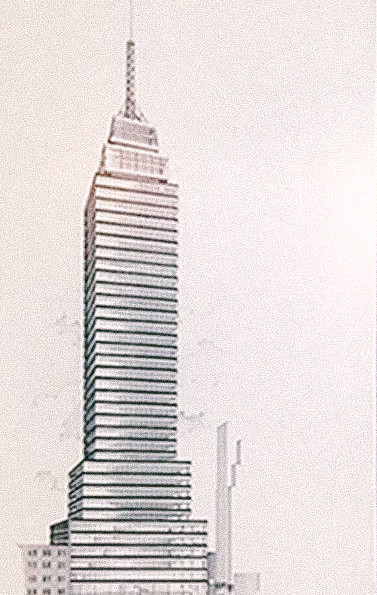
\includegraphics[scale=1.2]{Imagenes/Torre_Latino.jpg}
\end{figure}
\begin{tikzpicture}[overlay]
    \draw (7, 1.3) -- (7, 7) node [left, pos=1] {\small{$y$}};
    \draw (6, 1.3) -- (8, 1.3);
    \draw (6.7, 5.8) -- (7.3, 5.8);
    \draw [fill] (6.4, 5.8) circle (2pt);
\end{tikzpicture}
\end{frame}
\begin{frame}[plain]
\begin{figure}
\centering
\begin{tikzpicture}
    \draw (7, -1) -- (7, 7) node [left, pos=1] {\small{$y$}};

    \node at (2, 4) {\small{$a = -g = - \SI{9.81}{\meter\per\square\second}$}};
    \draw [-stealth, thick] (2.5, 3.5) -- (2.5, 2.5);

    \draw (6, -1) -- (8, -1);
    \draw (6.7, 5.8) -- (7.3, 5.8);
    \draw [fill] (6.4, 5.8) circle (2pt);
    
    \node at (5.4, 5.6) {\small{$v_{0} = 0$}};
    \node at (8.5, 5.6) {\small{$t_{0} = 0 \quad y_{0}=0$}};
    \pause

    \draw (6.7, 4.8) -- (7.3, 4.8);
    \draw [fill] (6.4, 4.8) circle (2pt);
    \node at (5.4, 4.6) {\small{$v_{1} =$ ?}};
    \draw [-stealth, thick] (6.4, 4.8) -- (6.4, 4.3);
    \node at (8.5, 4.6) {\small{$t_{1} = \SI{1}{\second} \quad y_{1}=$?}};
    \pause

    \draw (6.7, 3) -- (7.3, 3);
    \draw [fill] (6.4, 3) circle (2pt);
    \draw [-stealth, thick] (6.4, 3) -- (6.4, 2.3);
    \node at (5.4, 2.8) {\small{$v_{2} =$ ?}};
    \node at (8.5, 2.8) {\small{$t_{2} = \SI{2}{\second} \quad y_{2}=$?}};

    \pause

    \draw (6.7, 1) -- (7.3, 1);
    \draw [fill] (6.4, 1) circle (2pt);
    \draw [-stealth, thick] (6.4, 1) -- (6.4, -0.5);
    \node at (5.4, 0.8) {\small{$v_{3} =$ ?}};
    \node at (8.5, 0.8) {\small{$t_{3} = \SI{3}{\second} \quad y_{3}=$?}};

\end{tikzpicture}        
\end{figure}
\end{frame}
\begin{frame}
\frametitle{Preparando la solución}
Tomaremos el origen $O$ como el punto de partida y la dirección hacia arriba como positiva.
\\
\bigskip
\pause
La coordenada inicial $y_{0}$ y la velocidad inicial $v_{0}$ son ambas cero.
\end{frame}
\begin{frame}
\frametitle{Preparando la solución}
La aceleración es hacia abajo, en la dirección $y$ negativa, \pause así que:
\pause
\begin{align*}
a = - g = - \SI{9.81}{\meter\per\square\second}
\end{align*}
Recordemos que por definición $g$ siempre es positiva.
\end{frame}
\begin{frame}
\frametitle{Preparando la solución}
Por lo que nuestras incógnitas son los valores de $y$ y $v$ en los tres instantes que indica el enunciado.
\end{frame}
\begin{frame}
\frametitle{La expresión a utilizar}
Tenemos las siguientes expresiones:
\pause
\begin{eqnarray*}
\begin{aligned}
y &= v_{0} \, t + \dfrac{1}{2} \, a \, t^{2} \\[0.5em] \pause
v &= v_{0} + a \, t 
\end{aligned}
\end{eqnarray*}
\end{frame}
\begin{frame}
\frametitle{La expresión a utilizar}
En un instante $t$ después de que se suelta la moneda, su posición y velocidad son:
\pause
\begin{eqnarray*}
\begin{aligned}
y &= 0 + \dfrac{1}{2} (-g) \, t^{2} = \pause (\SI{-4.9}{\meter\per\square\second}) \, t^{2} \\[0.5em] \pause
v &= 0 + (-g) \, t = \pause (\SI{-9.8}{\meter\per\square\second}) \, t
\end{aligned}
\end{eqnarray*}
\end{frame}
\begin{frame}
\frametitle{Ocupando los tiempos}
Cuando $t = \SI{1}{\second}$, se tiene que:
\pause
\begin{eqnarray*}
\begin{aligned}
y &= (\SI{-4.9}{\meter\per\square\second}) \, (\SI{1}{\second})^{2} = \pause \SI{-4.9}{\meter} \\[0.5em] \pause
v &= (\SI{-9.8}{\meter\per\square\second}) (\SI{1}{\second}) = \pause \SI{-9.8}{\meter\per\second}
\end{aligned}
\end{eqnarray*}
\end{frame}
\begin{frame}
\frametitle{Los resultados}
Luego de \SI{1}{\second}, la moneda está \SI{4.9}{\meter} debajo del origen ($y$ es negativa), \pause y tiene una velocidad hacia abajo ($v$ es negativa) con magnitud de \SI{9.8}{\meter\per\second}.
\end{frame}
\begin{frame}
\frametitle{Evaluación continua}
La posición y velocidad a los \SI{2.0}{\second} y \SI{3.0}{\second} se obtienen de la misma manera.
\pause
Se puede demostrar que:
\begin{table}
\centering
\begin{tabular}{c | c | c}
Tiempo & Posición $(y)$& Velocidad $(v)$ \\ \hline
\SI{2.0}{\second} & \SI{-19.6}{\meter} & \SI{-19.6}{\meter\per\second} \\ \hline
\SI{3.0}{\second} & \SI{-44.1}{\meter} & \SI{-29.4}{\meter\per\second} \\ \hline
\end{tabular}
\end{table}
\end{frame}
\begin{frame}
\frametitle{Enunciado del Ejercicio 2}
Un niño lanza hacia abajo una piedra con una velocidad de \SI{2}{\meter\per\second} desde lo alto de un árbol de \SI{7}{\meter} de altura. 
\\
\bigskip
\pause
Calcula en cuánto tiempo llegará al piso y con qué velocidad lo hará.
\end{frame}
\begin{frame}
\frametitle{Resolviendo el ejercicio}
\textocolor{red}{Datos:}
\pause
\begin{align*}
v_{i} &= \SI{2}{\meter\per\second} \\[0.5em]
y &= \SI{7}{m} \\[0.5em]
g &= \SI{9.81}{\meter\per\square\second}
\end{align*}
\end{frame}
\begin{frame}
\frametitle{Resolviendo el ejercicio}
\textocolor{red}{Expresiones:}
\pause
\begin{eqnarray*}
\begin{aligned}
2 \, g \, y &= v_{f}^{2} - v_{i}^{2} \\[0.35em] \pause
v_{f}^{2} &= 2 \, g \, y + v_{i}^{2} \\[0.35em] \pause
v_{f} &= \sqrt{2 \, g \, y + v_{i}^{2}} \\[0.5em] \pause
v_{f} &= v_{i} + g \, t \\[0.35em] \pause
t &= \dfrac{v_{f} - v_{i}}{g}
\end{aligned}
\end{eqnarray*}
\end{frame}
\begin{frame}
\frametitle{Resolviendo el ejercicio}
\textocolor{red}{Sustitución:}
\pause
\begin{eqnarray*}
\begin{aligned}
v_{f} &= \sqrt{2 \left( \SI[per-mode=fraction]{9.81}{\meter\per\square\second}  \right) \left( \SI{7}{\meter} \right) + \left( \SI[per-mode=fraction]{2}{\meter\per\square\second} \right)^{2}} = \\[0.4em] \pause
v_{f} &= \SI{11.89}{\meter\per\second}
\end{aligned}
\end{eqnarray*}
\end{frame}
\begin{frame}
\frametitle{Resolviendo el ejercicio}
\textocolor{red}{Sustitución:}
\pause
\begin{eqnarray*}
\begin{aligned}
t &= \dfrac{\SI[per-mode=fraction]{11.89}{\meter\per\second} - \SI[per-mode=fraction]{2}{\meter\per\second}}{\SI[per-mode=fraction]{9.81}{\meter\per\square\second}} \\[0.4em] \pause
t &= \SI{1}{\second}
\end{aligned}
\end{eqnarray*}
\end{frame}
\end{document}